\documentclass[11pt,a4paper]{article}

\usepackage[T1]{fontenc}
\usepackage[utf8]{inputenc}
\usepackage[spanish,es-nodecimaldot,es-noshorthands]{babel}
\usepackage[sc]{mathpazo}
\linespread{1.05}
\usepackage{amsmath,amssymb}
\usepackage{graphicx,subcaption,booktabs}
\usepackage{float}
\usepackage[margin=2.5cm]{geometry}
\usepackage{microtype}
\usepackage{titlesec}
\usepackage{fancyhdr}
\usepackage[font=small,labelfont=bf]{caption}
\usepackage[colorlinks=true, linkcolor=blue]{hyperref}


% Secciones con separador
\titleformat{\section}{\Large\bfseries}{\thesection.}{0.6em}{}[{\titlerule[0.6pt]}]
\titlespacing*{\section}{0pt}{1.6em}{0.9em}

% Encabezado
\pagestyle{fancy}
\fancyhf{}
\fancyhead[L]{\small\textsc{Macroeconomía Internacional Cuantitativa}}
\fancyhead[R]{\small Problem Set 2 --- Problema de la torta}
\fancyfoot[C]{\small\thepage}
\renewcommand{\headrulewidth}{0.4pt}


\begin{document}

\begin{titlepage}
    \centering
    \vspace*{1cm}
    
\includegraphics[width=0.7\textwidth]{logo_udesa.pdf}\\[2cm]

    {\scshape\Large Maestría en Economía \par}
    \vspace{0.5cm}
    {\scshape\large Macroeconomía Internacional Cuantitativa \par}
    \vspace{1cm}

    \rule{\linewidth}{0.5pt}\\[0.4cm]
    {\huge\bfseries Problem Set 2\par}
    \vspace{0.1cm}
    {\Large Problema de la torta\par}
    \rule{\linewidth}{0.5pt}\\[1cm]

    {\large
    Martín A. Fradkin \par}

    \vfill

    {\large Profesor: Francisco Roldán \par}
    \vspace{0.5cm}
    {\large \today \par}

\end{titlepage}

% ==================================================================
% INTRODUCCIÓN
% ==================================================================
\section*{Modelo y resolución numérica}

Un agente dispone de una torta $k$ que rinde un interés $r$ y decide cuánto consumir hoy y cuánto conservar para el período siguiente:
\[
v(k)=\max_{k'}\; u\big(k(1+r)-k'\big)+\beta\, v(k'),\qquad u(c)=\frac{c^{1-\gamma}-1}{1-\gamma},
\]
con los parámetros por defecto del código del curso: $\beta=0.96$, $\gamma=2$ y $r=0.02$. Con preferencias CRRA el problema es homogéneo en $k$ y la solución consiste en consumir siempre la misma fracción de la torta disponible:
\begin{equation}\label{eq:theta}
c(k)=\theta k,\qquad \theta=(1+r)-\big[\beta(1+r)\big]^{1/\gamma}=0.0305 .
\end{equation}
Esta forma cerrada sirve como referencia para evaluar las soluciones numéricas. El modelo se resolvió por iteración de la función de valor con los dos algoritmos del curso: \texttt{vfi!}, que restringe la elección de $k'$ a los puntos de la grilla, y \texttt{vfi\_itp!}, que elige $k'$ en forma continua e interpola linealmente $v$ entre los puntos de la grilla. Se usaron la grilla por defecto, de $N_k=20$ puntos equiespaciados en $(0,1]$, y una grilla fina de $N_k=1000$ puntos.

% ==================================================================
\section{Funciones de consumo}
\label{sec:funciones}
% ==================================================================

\subsection{Resolución del modelo}
\label{sec:resolucion}

Se crearon objetos \texttt{CakeEating} con los parámetros por defecto ($\beta=0.96$, $\gamma=2$, $r=0.02$, torta inicial $k_0=1$) y se resolvieron con ambos algoritmos, sobre la grilla por defecto de $N_k=20$ puntos y sobre una grilla de $N_k=1000$ puntos. En los cuatro casos la iteración convergió en 374 pasos, con una distancia relativa entre iteraciones sucesivas inferior a $10^{-8}$. La forma cerrada \eqref{eq:theta} indica que el agente debe comer el $3.05\%$ de su torta en cada período ($\theta=0.0305$) y conservar el resto ($k'/k=1+r-\theta=0.9895$).

\subsection{Función de consumo}
\label{sec:consumo}

\begin{figure}[h!]
\centering
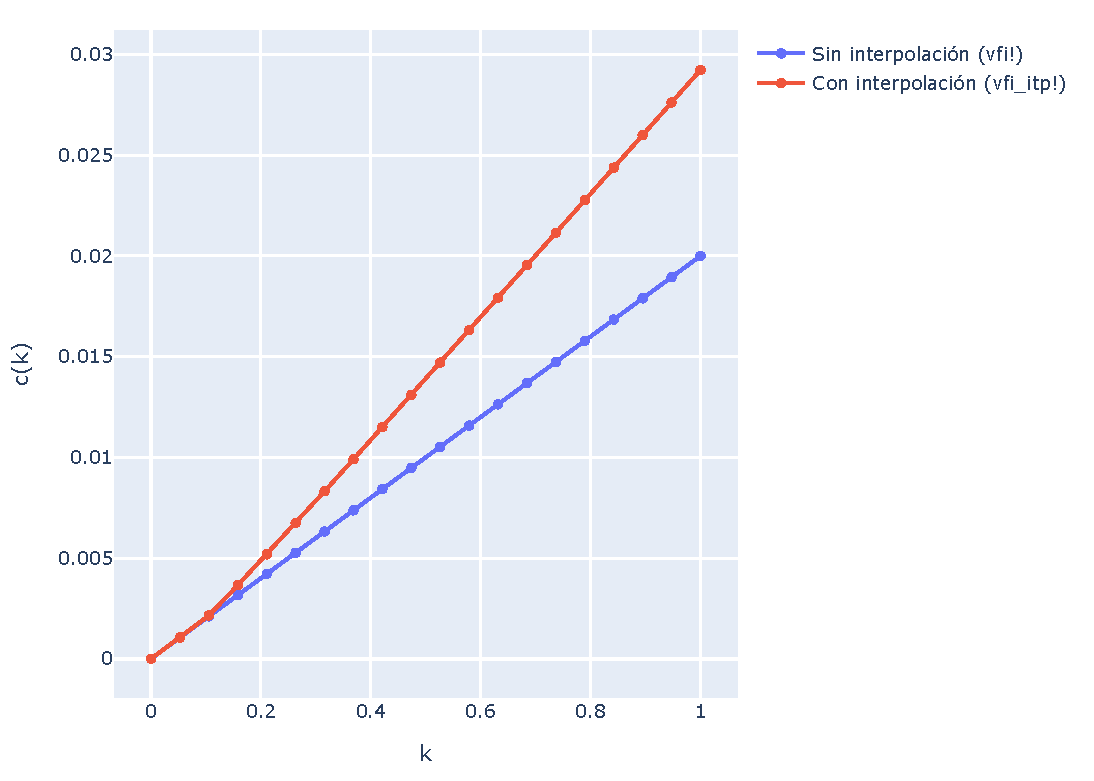
\includegraphics[width=0.6\textwidth]{c_k.pdf}
\caption{Consumo en función de la torta disponible, $N_k=20$.}
\label{fig:c}
\end{figure}

Con ambos métodos el consumo es una recta que parte del origen (Figura~\ref{fig:c}). La pendiente de esa recta es la fracción de la torta que el agente come en cada período, $c/k$, que es justamente lo que la teoría predice y lo que permite comparar los métodos. El gráfico en niveles es poco informativo por dos razones. En primer lugar, no permite verificar la predicción central del modelo: que esa fracción sea la misma para cualquier tamaño de torta (esto porque una curva levemente doblada es indistinguible de una recta). Esto es apreciable en la solución con interpolación, que en la Figura~\ref{fig:c} parece una recta aunque la fracción consumida varía entre $0.020$ y $0.029$ según $k$, como se ve en el inciso~\ref{sec:consumorelativo}. En segundo lugar, como todas las curvas parten de cero, la distancia vertical entre ellas es proporcional a $k$: es nula para torta chica y sólo se aprecia cerca de $k=1$, donde los consumos son $0.020$ sin interpolación y $0.029$ con interpolación, contra $0.0305$ según la teoría.

\subsection{Consumo relativo}
\label{sec:consumorelativo}

\begin{figure}[h!]
\centering
\begin{subfigure}{.49\textwidth}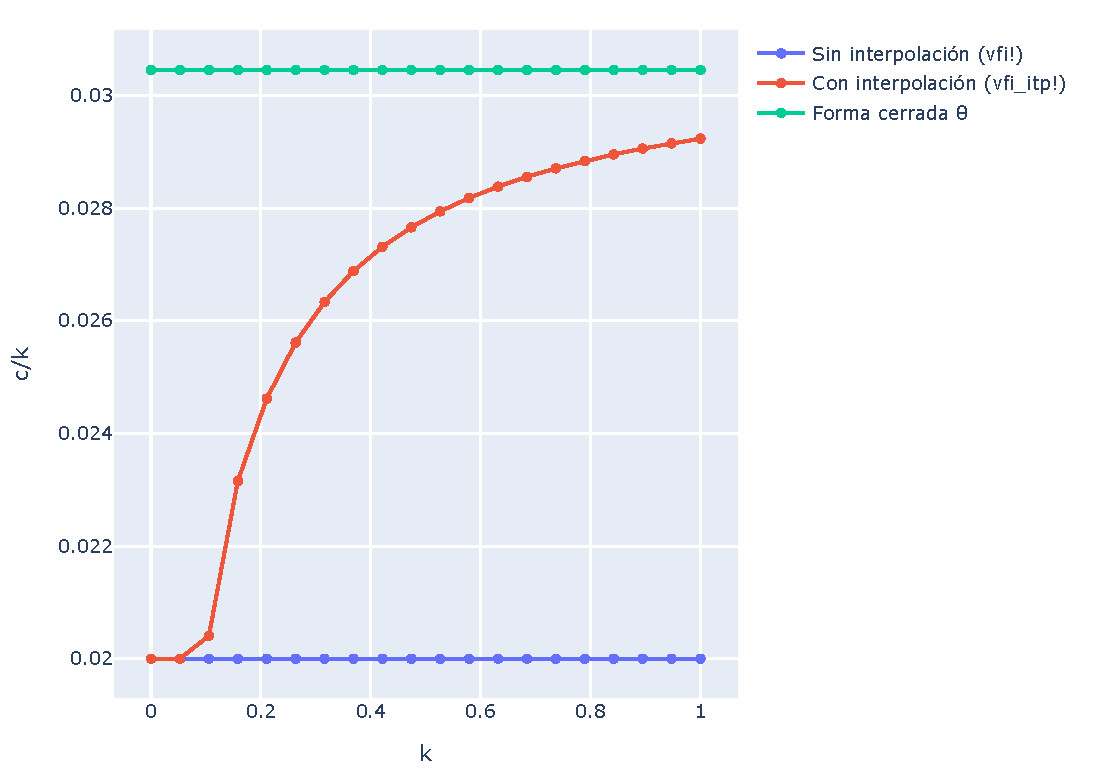
\includegraphics[width=\linewidth]{ck_k_N20.pdf}\caption{$N_k=20$}\end{subfigure}
\begin{subfigure}{.49\textwidth}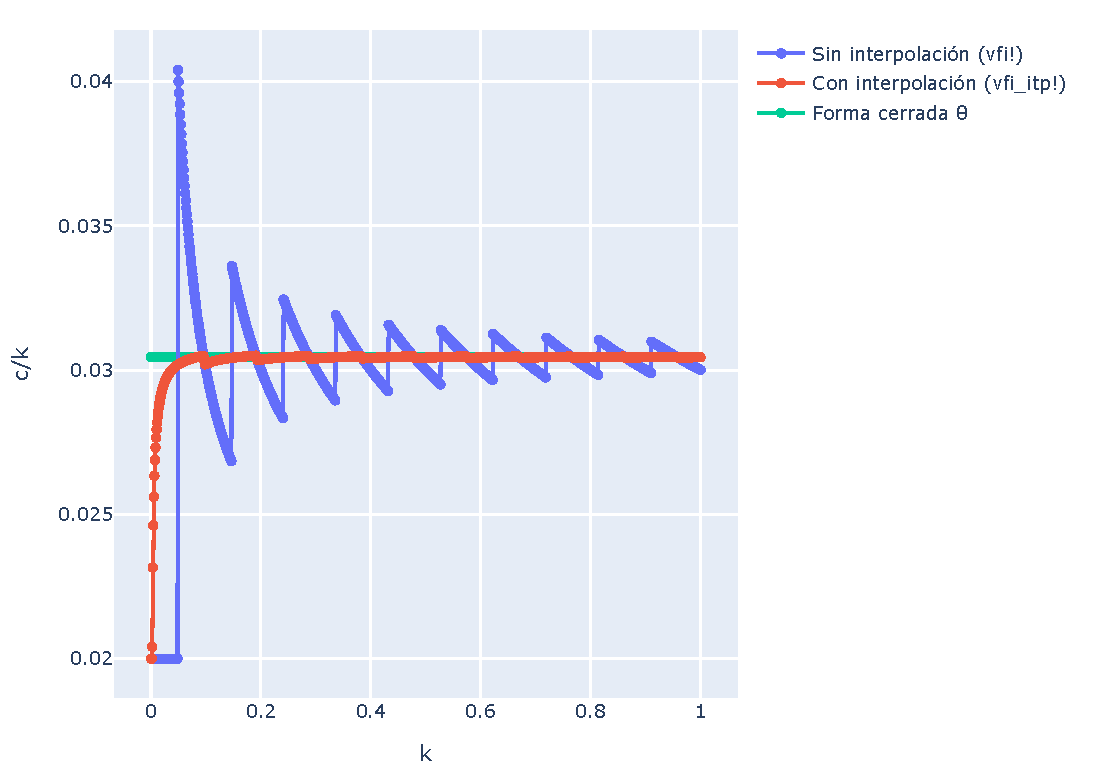
\includegraphics[width=\linewidth]{ck_k_N1000.pdf}\caption{$N_k=1000$}\end{subfigure}
\caption{Fracción de la torta consumida en cada período, $c/k$, en función de la torta disponible.}
\label{fig:ck}
\end{figure}

Al dividir por $k$, la fracción consumida pasa a leerse directamente en el eje vertical. Según la teoría debería ser una línea horizontal en $\theta=0.0305$, y cualquier dependencia respecto de $k$ revela un error numérico. Con la grilla por defecto (Figura~\ref{fig:ck}a) ninguno de los dos métodos reproduce ese resultado:

\paragraph{\textit{Sin interpolación}.} El agente consume $c/k=0.02=r$ para cualquier torta: come exactamente los intereses y la torta nunca se achica. La causa es que $k'$ debe ser un punto de la grilla, separados entre sí por $0.053$. Con $k=1$, el agente querría conservar $0.99$, pero el punto inmediatamente inferior a $1$ es $0.947$. Llegar a ese punto implicaría recortar la torta cinco veces más de lo deseado, de modo que prefiere no achicarla. El valor resultante es el de consumir $0.02$ para siempre, $u(0.02)/(1-\beta)=-1225$ (exactamente $v(1)$ en el Cuadro~\ref{tab:v}).
\paragraph{\textit{Con interpolación}.} El agente puede elegir cualquier $k'$, pero consume menos de lo óptimo: $c/k$ va de $0.025$ en $k=0.2$ a $0.029$ en $k=1$. Entre dos puntos de la grilla, $v$ se aproxima con una recta cuya pendiente es la pendiente promedio de $v$ en ese tramo. Como $v$ es cóncava, la pendiente verdadera cerca del extremo derecho del tramo (donde se ubica el $k'$ óptimo) es menor que ese promedio. El algoritmo sobrestima entonces cuánto vale conservar una unidad más de torta, y el agente ahorra de más. El error crece al acercarse a cero, porque allí la curvatura de $v$ es mayor y la recta se aparta más de la función.

\subsection{Ahorro relativo}
\label{sec:ahorro}

\begin{figure}[h!]
\centering
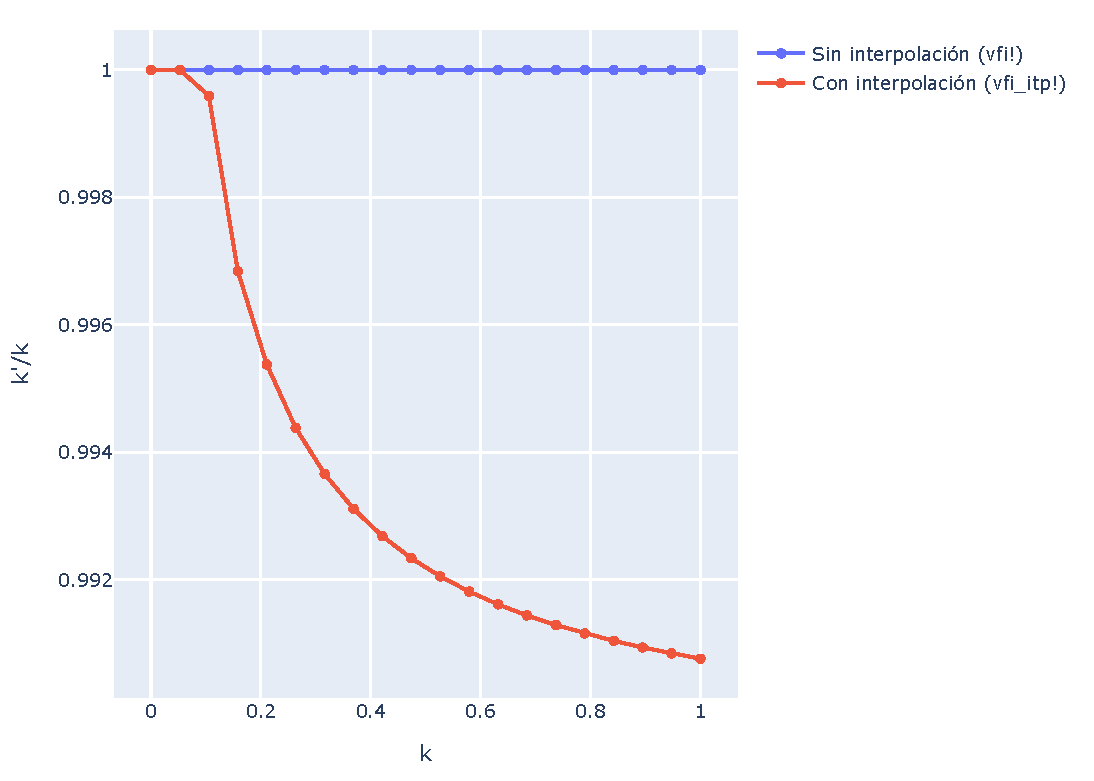
\includegraphics[width=0.6\textwidth]{kk_k.pdf}
\caption{Fracción de la torta conservada para el período siguiente, $k'/k$, $N_k=20$.}
\label{fig:kk}
\end{figure}

Por la restricción presupuestaria, $k'/k=(1+r)-c/k$: el ahorro relativo es la imagen especular del consumo relativo y no agrega información independiente (Figura~\ref{fig:kk}). Lo que hace visible es que, sin interpolación, $k'/k=1$ en todos los puntos, es decir, que con 20 puntos de grilla el agente nunca empieza a comerse la torta.

Al aumentar la cantidad de puntos y alejarse del cero, $c/k$ se vuelve constante, que es la forma que predice la teoría (Figura~\ref{fig:ck}b). Con $N_k=1000$ y $k\geq0.2$, la solución con interpolación se ubica entre $0.0304$ y $0.0305$, sobre la forma cerrada. La solución sin interpolación oscila en forma de serrucho entre $0.028$ y $0.032$ alrededor de $\theta$.

Según la forma cerrada, la torta del período siguiente es $0.9895\,k$\footnote{$k'=k(1+r)-c=1.02k-0.0305k=0.9895k$.}, de modo que se reduce en $0.0105\,k$ por período. Sin interpolación, el agente sólo puede elegir $k'$ entre puntos de la grilla separados por $0.001$ y, al elegir el punto más conveniente, se equivoca en $k'$ hasta en medio espaciado ($0.0005$). Como $c=k(1+r)-k'$, ese error se traslada uno a uno al consumo. Sin embargo, en la fracción $c/k$ ese error se divide por $k$ y pesa $0.0005/k$: es chico con torta grande y crece a medida que la torta se achica. Para $k\geq0.2$, $c/k$ se ubica entre $0.028$ y $0.032$, y el rango se va comprimiendo a medida que crece $k$. Con $k=0.05$ la reducción deseada es de medio espaciado, y el agente sólo puede comerse los intereses sin reducir la torta ($k'=0.05;\ c=0.001;\ c/k=0.02$) o reducirla un espaciado entero ($k'=0.049;\ c=0.002;\ c/k=0.04$), por lo que las oscilaciones alcanzan esos valores cerca de cero. La forma de serrucho surge porque, al aumentar $k$, el $k'$ elegido se mantiene en el mismo punto de la grilla hasta que conviene saltar al siguiente. En el primer punto de la grilla, $k=10^{-6}$, ambas reglas dan $c/k=0.02$ porque no existe un punto inferior y el agente está obligado a conservar la torta.

\paragraph{Conclusión.} Con utilidad CRRA el agente consume siempre la misma fracción de la torta que le queda, sin importar cuánta le quede. La solución numérica reproduce ese resultado sólo con una grilla fina y eligiendo $k'$ en forma continua. Con pocos puntos, la grilla no sólo introduce imprecisión, sino que puede cambiar la decisión por completo: si el recorte deseado es menor que la distancia entre dos puntos, el agente deja de comerse la torta.

% ==================================================================
\section*{Modos de resolución}
% ==================================================================

\begin{figure}[h!]
\centering
\begin{subfigure}{.49\textwidth}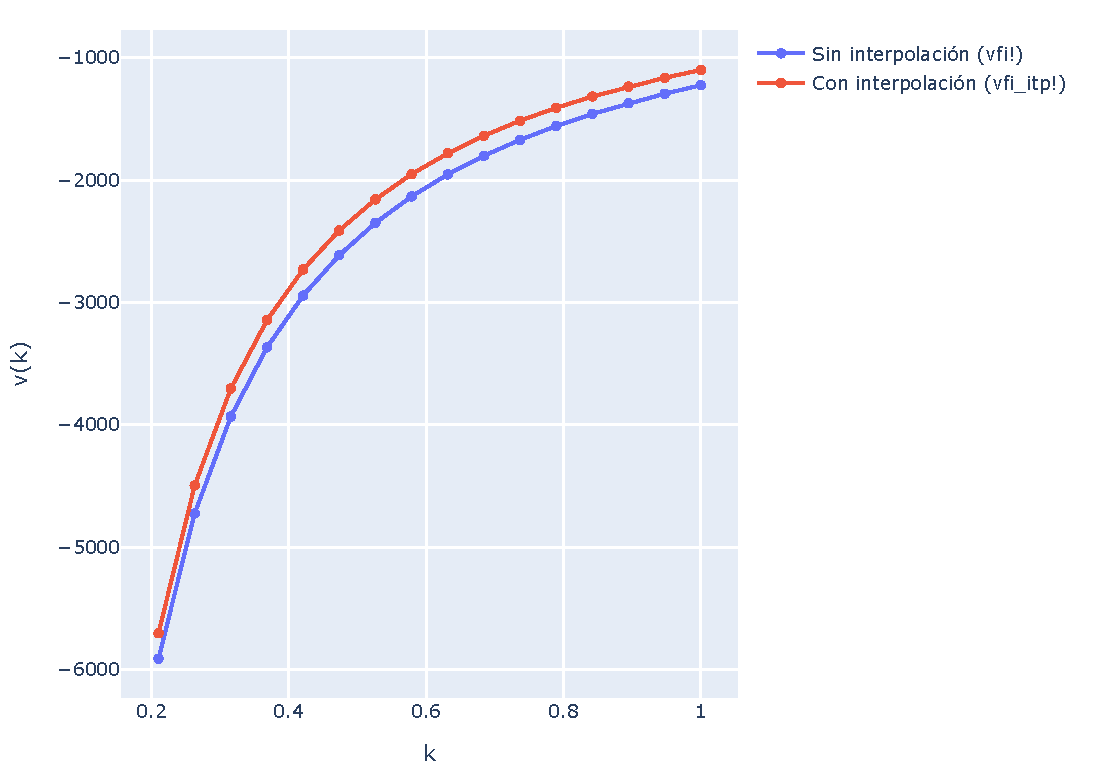
\includegraphics[width=\linewidth]{v_k_N20.pdf}\caption{$N_k=20$}\end{subfigure}
\begin{subfigure}{.49\textwidth}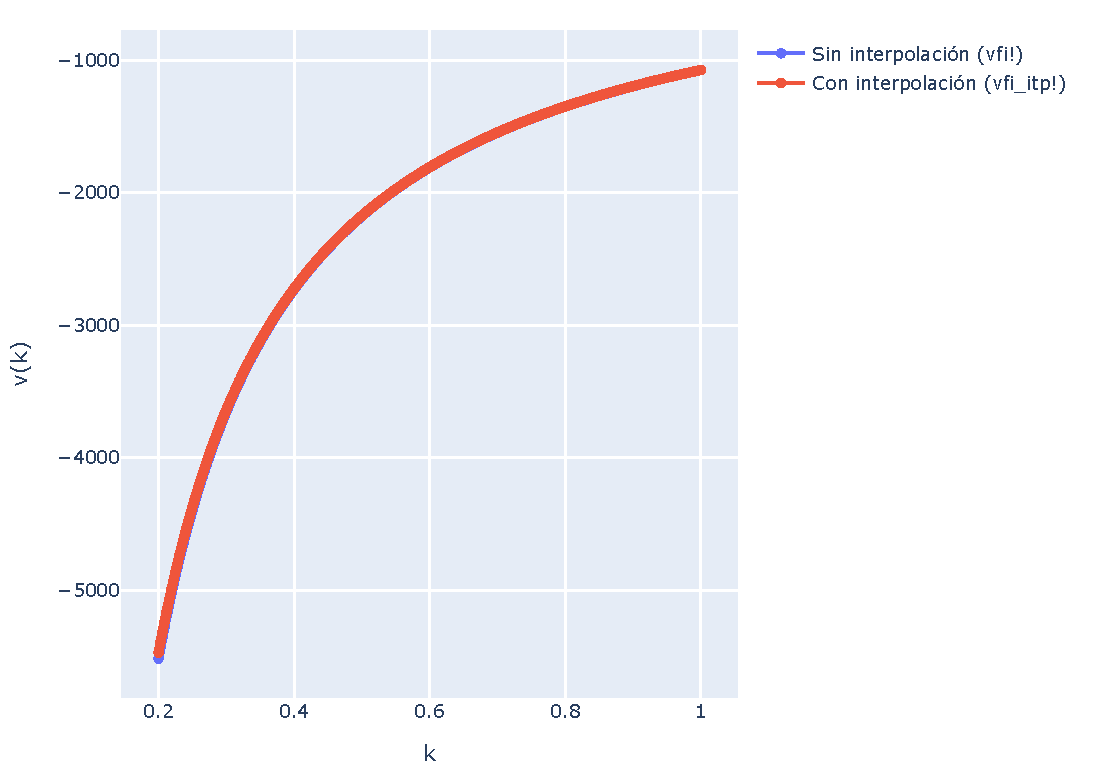
\includegraphics[width=\linewidth]{v_k_N1000.pdf}\caption{$N_k=1000$}\end{subfigure}
\caption{Función de valor en función de la torta disponible, $k\geq0.2$.}
\label{fig:v}
\end{figure}

\begin{table}[h!]
\centering
\begin{tabular}{lcc}
\toprule
 & $N_k=20$ & $N_k=1000$\\
\midrule
Sin interpolación (\texttt{vfi!})      & $-1225.00$ & $-1075.07$\\
Con interpolación (\texttt{vfi\_itp!}) & $-1100.26$ & $-1074.74$\\
\midrule
Forma cerrada & \multicolumn{2}{c}{$-1074.75$}\\
\bottomrule
\end{tabular}
\caption{Función de valor evaluada en $k=1$.}
\label{tab:v}
\end{table}

Los dos algoritmos no dan el mismo resultado. La diferencia está en el conjunto de valores de $k'$ entre los que puede elegir el agente: sin interpolación, sólo los puntos de la grilla; con interpolación, cualquier valor del intervalo, a costa de evaluar $v$ entre puntos de la grilla mediante una recta.

\paragraph{Función de valor.} Sin interpolación, $v$ queda por debajo en todo el rango (Figura~\ref{fig:v}a). Elegir entre menos opciones no puede dar más bienestar que elegir entre todas. Con 20 puntos, $v(1)$ se ubica 150 unidades por debajo de la forma cerrada, contra 26 con interpolación (Cuadro~\ref{tab:v}). Con 1000 puntos ambos métodos se acercan a la solución exacta, pero no por igual: el error sin interpolación es de $0.32$ y con interpolación es prácticamente nulo.

\paragraph{Regla de decisión relativa.} En $c/k$ las diferencias son mucho más visibles que en $v$. Con $N_k=1000$ las dos funciones de valor son indistinguibles a simple vista, mientras que la fracción consumida sin interpolación se aparta hasta un $7\%$ de $\theta$ para $k\geq0.2$ (Figura~\ref{fig:ck}b).
Esto se debe a que en el óptimo la derivada del objetivo respecto de $k'$ es cero, alrededor del máximo el objetivo es casi plano, y desviarse de él reduce el valor en una magnitud proporcional al cuadrado de la desviación\footnote{Para desvíos suficientemente bajos, el cuadrado del desvío es menor que el desvío mismo, haciendo que la diferencia observada en la decisión $(k';\,c/k)$ sea mayor que la percibida en la función valor $v$.}. Con $k=1$, el método discreto consume $0.030$ en lugar de $0.0305$, un error de $1.6\%$ en la decisión, mientras que el error en $v(1)$ es de $0.03\%$ ($-1075.07$ contra $-1074.75$).
Errores apreciables en la decisión producen así errores despreciables en el valor $(v)$.

\paragraph{Conclusión.} El método sin interpolación falla porque restringe las decisiones a los puntos de la grilla; el método con interpolación falla porque aproxima $v$ con rectas entre esos puntos. El segundo error es menor y desaparece más rápido al afinar la grilla. Como la función de valor apenas cambia ante errores en la decisión, una solución numérica debe evaluarse a partir de la regla de decisión. Una función de valor que coincide con la teórica puede corresponder a decisiones visiblemente equivocadas.


% ==================================================================
\section*{Para pensar}
% ==================================================================
\subsection*{Opción 1: decidir con la función de valor exacta}
Con utilidad CRRA el problema con torta $k$ es el problema con torta unitaria multiplicado por $k$, de modo que la función de valor tiene la forma $v(k)=\tilde v\,k^{1-\gamma}$. Reemplazando esta forma en la ecuación de Bellman y evaluando en $k=1$, la incógnita deja de ser una función y pasa a ser un número:
\[
\tilde v=\max_{k'}\;\frac{(1+r-k')^{1-\gamma}}{1-\gamma}+\beta\,\tilde v\,(k')^{1-\gamma}.
\]
Iterando esta ecuación a partir de $\tilde v=0$ se obtiene $\tilde v=-1099.75$. Es el mismo valor que resulta de sumar la utilidad descontada de la trayectoria óptima $c_t=\theta k\,g^t$, con $g=1+r-\theta$:
\[
\tilde v=\frac{\theta^{1-\gamma}}{(1-\gamma)\,(1-\beta g^{1-\gamma})}=-\frac{1}{\theta\,(1-\beta/g)}=-1099.75 .
\]
La utilidad del código \texttt{cakeeating.jl}, $(c^{1-\gamma}-1)/(1-\gamma)$, suma a la función de valor la constante $-1/[(1-\gamma)(1-\beta)]=25$. Con ella, $v(1)=25+\tilde v=-1074.75$, el valor de referencia del Cuadro~\ref{tab:v}. Como la constante es la misma para todas las opciones, no altera la decisión. Con $\tilde v$ se calculó el consumo en cada punto de la grilla, eligiendo $k'$ en forma continua para maximizar $u(k(1+r)-k')+\beta\tilde v(k')^{1-\gamma}$.

\begin{figure}[h!]
\centering
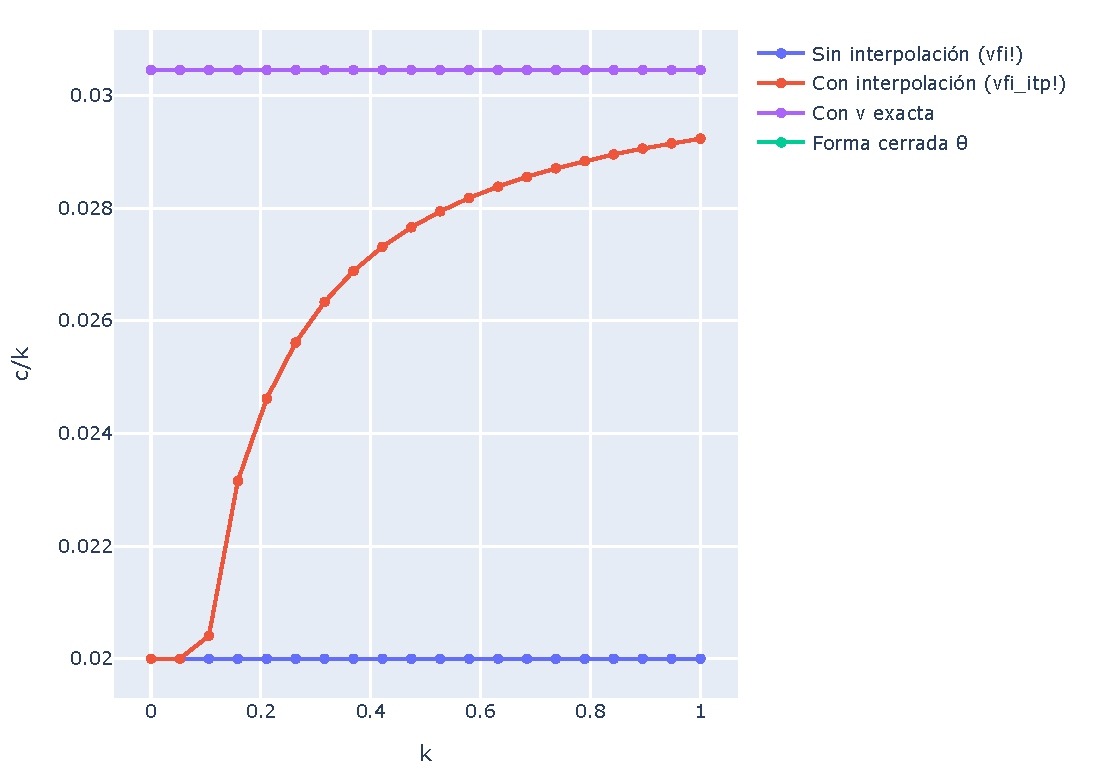
\includegraphics[width=0.6\textwidth]{ck_vt.pdf}
\caption{Fracción de la torta consumida con la función de valor exacta y con los dos algoritmos, $N_k=20$.}
\label{fig:vt}
\end{figure}

El resultado no es igual al del inciso~\ref{sec:consumorelativo}. Con la función de valor exacta, $c/k=0.030455$ en todos los puntos de la grilla, y también en $k=10^{-6}$, que coincide con $\theta$ hasta el sexto decimal (Figura~\ref{fig:vt}). El mismo resultado se obtiene con $N_k=1000$. Las diferencias con las soluciones de la Sección~\ref{sec:funciones} se concentran donde éstas aproximaban peor a $v$. Con la grilla gruesa, el método discreto consume sólo los intereses y el método con interpolación consume entre $0.025$ y $0.029$ de la torta (inciso~\ref{sec:consumorelativo}). En el primer punto de la grilla, ambos caen a $c/k=0.02$ porque no pueden elegir $k'$ por debajo del mínimo de la grilla (inciso~\ref{sec:ahorro}). Con la función de valor exacta la grilla deja de influir en la decisión: sólo determina en qué valores de $k$ se calcula el consumo, pero no restringe ni distorsiona la elección de $k'$.

\paragraph{Conclusión.} La optimización no es la fuente del error numérico. Cuando el agente conoce el valor verdadero de cada torta posible para mañana, elige exactamente lo que predice la teoría con cualquier grilla. Todo el error de los algoritmos de la Sección~\ref{sec:funciones} proviene de tener que aproximar la función de valor a partir de un número finito de puntos.



% ==================================================================
\subsection*{Opción 2: la torta en logaritmos}
% ==================================================================

Se reescribió el problema con $x=\log k$ como variable de estado, sobre una grilla equiespaciada en $x\in[-10,0]$, con restricción presupuestaria $c+e^{x'}=e^{x}(1+r)$. En términos de $k$, los puntos van de $e^{-10}=0.000045$ a $1$ y se acumulan cerca de cero: con $N_x=20$, sólo 4 quedan por encima de $k=0.2$. La función de valor se interpola linealmente en $x$ y $x'$ se elige en forma continua. Se resolvió con $N_x=20$ y $N_x=1000$, primero restringiendo $x'$ a la grilla y luego permitiendo, mediante extrapolación lineal, elegir $x'$ por debajo de $-10$.

\begin{figure}[H]
\centering
\begin{subfigure}{.49\textwidth}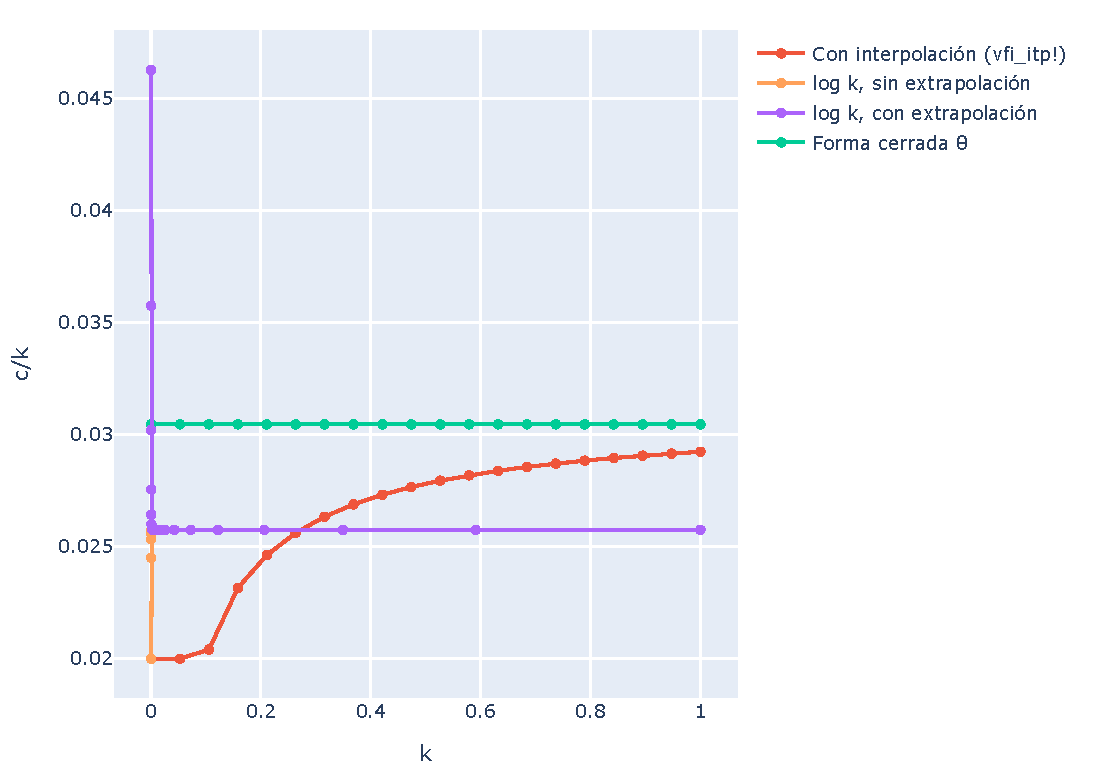
\includegraphics[width=\linewidth]{ck_log_N20.pdf}\caption{$N=20$}\end{subfigure}
\begin{subfigure}{.49\textwidth}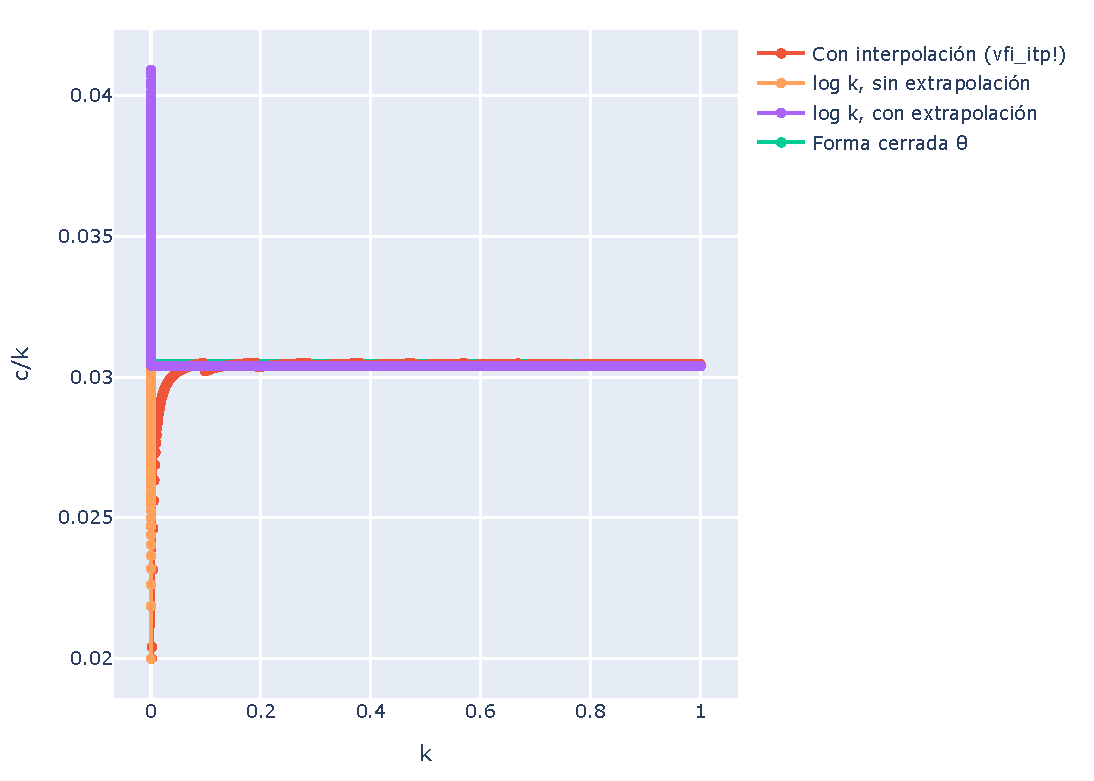
\includegraphics[width=\linewidth]{ck_log_N1000.pdf}\caption{$N=1000$}\end{subfigure}\\[4pt]
\begin{subfigure}{.49\textwidth}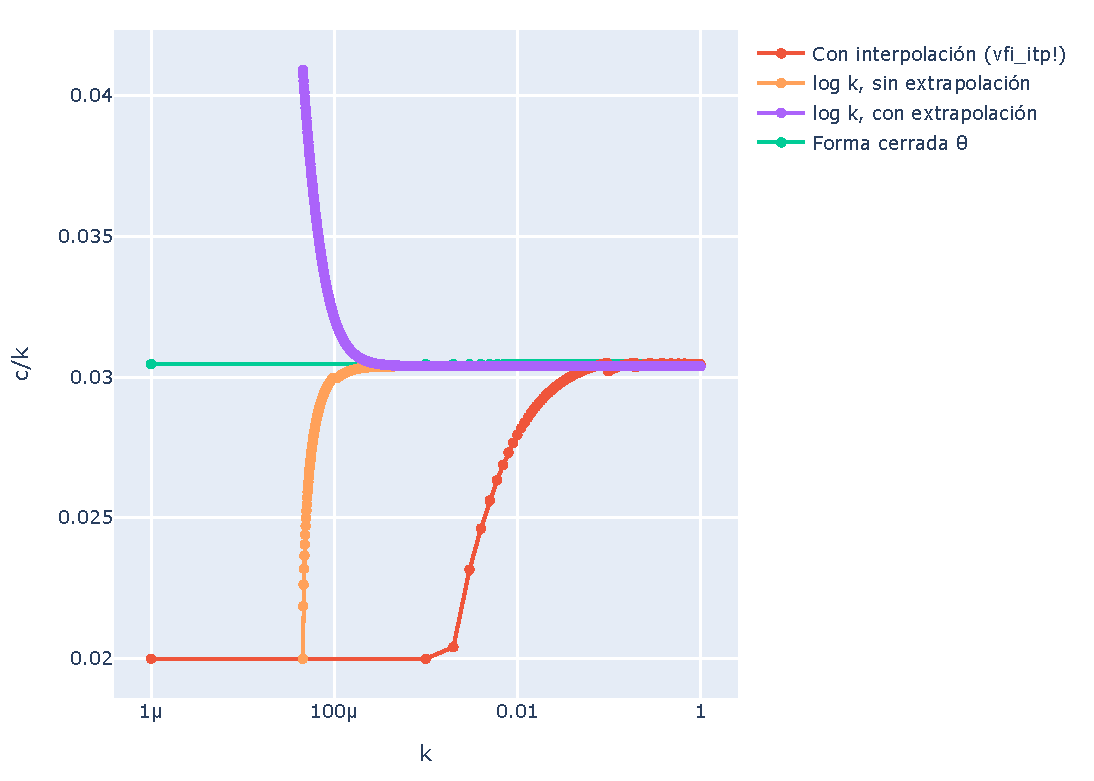
\includegraphics[width=\linewidth]{ck_log_N1000_logx.pdf}\caption{$N=1000$, eje de $k$ en escala logarítmica}\end{subfigure}
\caption{Fracción de la torta consumida con la grilla en $\log k$, sin y con extrapolación, y con la grilla en $k$ del inciso~\ref{sec:consumorelativo}. Sin y con extrapolación las reglas coinciden salvo en los primeros puntos de la grilla.}
\label{fig:log}
\end{figure}

\begin{table}[H]
\centering
\begin{tabular}{lcccc}
\toprule
 & $v(1)$ & $c/k$ en $k=1$ & $c/k$ en $k_{\min}$ & desvío $>1\%$\\
\midrule
\multicolumn{5}{l}{\textit{$N=20$}}\\
Interpolación $(k)$                    & $-1100.26$ & 0.0292  & 0.0200 & --\\
Interpolación $(\log k)$               & $-1162.09$ & 0.0257  & 0.0200 & toda la grilla\\ 
Interpolación $(\log k)$, extrapolando & $-1162.10$ & 0.0257  & 0.0463 & toda la grilla\\
\midrule
\multicolumn{5}{l}{\textit{$N=1000$}}\\
Interpolación $(k)$                    & $-1074.74$ & 0.0305  & 0.0200 & $k<0.045$\\
Interpolación $(\log k)$               & $-1074.82$ & 0.0304  & 0.0200 & $k<0.00013$\\
Interpolación $(\log k)$, extrapolando & $-1074.83$ & 0.0304  & 0.0409 & $k<0.00017$\\
\midrule
Forma cerrada                           & $-1074.75$ & 0.0305  & 0.0305 & --\\
\bottomrule
\end{tabular}
\caption{Resultados con la grilla en $k$ y en $\log k$. $k_{\min}$ es el primer punto de cada grilla: $10^{-6}$ en $k$ y $e^{-10}$ en $\log k$. La última columna indica hasta qué torta $c/k$ se aparta más de un $1\%$ de $\theta$.}
\label{tab:log}
\end{table}

\paragraph{Forma de la regla.} Con la grilla en $\log k$, la fracción consumida es constante en toda la grilla, salvo en los primeros puntos (Figura~\ref{fig:log}a y~\ref{fig:log}b). Es la forma que predice la teoría, y no se obtenía con la grilla en $k$, donde $c/k$ dependía del tamaño de la torta. La razón es que la función de valor verdadera, $v=25-1.10\,e^{-x}$, tiene la misma forma en cada tramo de una grilla equiespaciada en $x$, sólo que a distinta escala, y el $x'$ óptimo, $x-0.0105$, cae siempre en la misma posición dentro de su tramo. El error de aproximar $v$ con rectas es entonces la misma proporción en todos los puntos, y la distorsión de la decisión también. La grilla en logaritmos traslada al algoritmo la homogeneidad de la utilidad CRRA: el error no desaparece, pero deja de depender de $k$. Con $N=20$ la regla es plana pero se ubica un $15\%$ por debajo de $\theta$ ($c/k=0.0257$); con $N=1000$ el desvío lejos del cero es de $0.22\%$, similar al de la grilla en $k$.

\paragraph{Mejor y peor.} Concentrar los puntos cerca de cero mejora la regla donde la grilla en $k$ era menos precisa. Con $N=1000$, la zona en la que $c/k$ se aparta más de un $1\%$ de $\theta$ se reduce de $k<0.045$ a $k<0.00013$ (Figura~\ref{fig:log}c y Cuadro~\ref{tab:log}). Esos puntos se obtienen a costa de los tramos con torta grande. Con $N=20$ y sólo 4 puntos por encima de $k=0.2$, en $k=1$ el agente consume $0.0257$, contra $0.0292$ con la grilla en $k$, y el error en $v(1)$ pasa de 26 a 87 unidades.

\paragraph{Extrapolación.} Sin extrapolación, en el primer punto de la grilla el agente no puede elegir $x'<-10$ y consume sólo los intereses ($c/k=0.02$), como en la Sección~\ref{sec:funciones}. La extrapolación le permite achicar la torta por debajo de ese punto, pero evalúa $v$ prolongando con una recta el último tramo, mientras que la función verdadera cae exponencialmente al reducir $x$. El algoritmo subestima entonces cuánto se pierde al achicar la torta, y el agente consume de más: $c/k=0.041$ con $N=1000$. El desvío en el extremo inferior cambia de signo, de $-34\%$ a $+34\%$, pero la zona afectada no se reduce ($k<0.00017$).

\paragraph{Conclusión.} Elegir dónde ubicar los puntos de la grilla importa tanto como cuántos usar. Una grilla equiespaciada en $\log k$ respeta la homogeneidad del problema y produce una regla de consumo con la forma correcta, una fracción constante de la torta, aunque con pocos puntos esa fracción esté sesgada. La extrapolación no resuelve el problema del extremo inferior: sólo reemplaza el supuesto de que el agente no puede bajar de la grilla por el de que, por debajo de ella, la función de valor sigue una recta.



% ==================================================================
\section{Simulador de torta}
\label{sec:simulador}
% ==================================================================

Se programó una función que toma un modelo resuelto, un horizonte $T$ y una torta inicial $k_0$, y devuelve las sucesiones $\{c_t,k_t\}_{t=0}^{T}$. Como las reglas de consumo y de ahorro sólo están calculadas en los puntos de la grilla y la torta simulada en general cae entre ellos, ambas reglas se interpolan linealmente. En cada período, a partir de $k_t$ la regla de consumo da $c_t$ y la de ahorro da $k_{t+1}$. Se usaron $T=250$ y $k_0=1$, el máximo de la grilla. La referencia es la forma cerrada con interés: la torta se reduce en la proporción constante $g=1+r-\theta=0.9895$ por período y el consumo es una fracción fija de ella,
\[
k_t=k_0\,g^{t},\qquad c_t=\theta\,k_t .
\]


\subsection{Trayectorias simuladas}

\begin{figure}[h!]
\centering
\begin{subfigure}{.49\textwidth}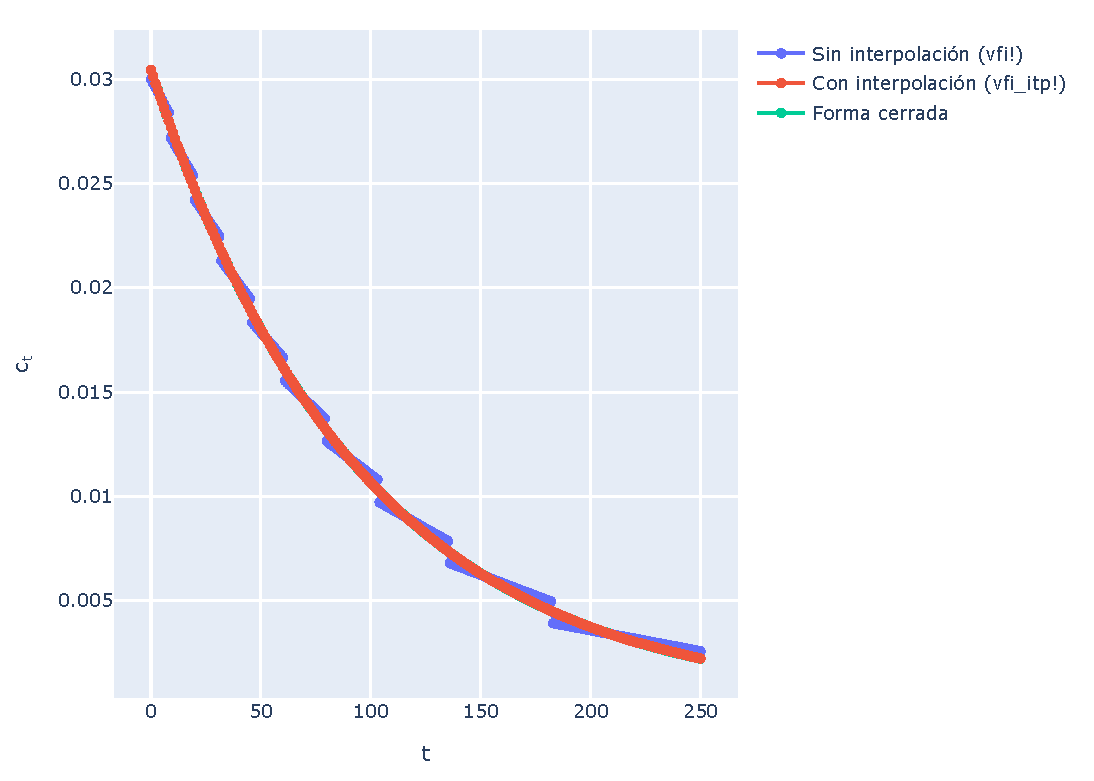
\includegraphics[width=\linewidth]{sim_c.pdf}\caption{Consumo $c_t$}\end{subfigure}
\begin{subfigure}{.49\textwidth}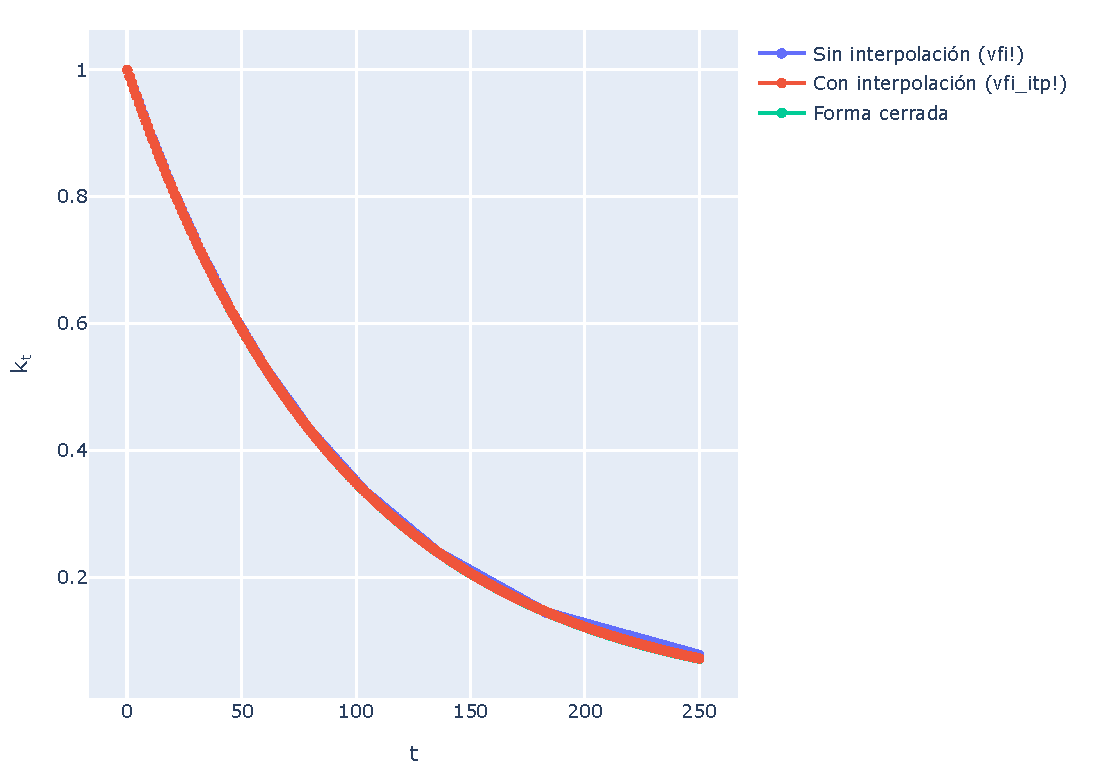
\includegraphics[width=\linewidth]{sim_k.pdf}\caption{Torta $k_t$}\end{subfigure}
\caption{Trayectorias simuladas con $N_k=1000$ y forma cerrada, $k_0=1$.}
\label{fig:sim}
\end{figure}

Con interpolación y $N_k=1000$, la simulación reproduce la forma cerrada (Figura~\ref{fig:sim}). La torta y el consumo caen al mismo ritmo, $1.05\%$ por período: la torta pasa de $1$ a $0.073$ y el consumo de $0.0305$ a $0.0022$. La trayectoria tiene la misma forma que la vista en clase, una caída geométrica del consumo, pero no los mismos valores, porque aquella supone $r=0$. Con interés, la torta guardada crece mientras se espera para comerla. Por eso el consumo cae más lento ($1.05\%$ por período contra $1-\beta^{1/\gamma}=2.02\%$ con $r=0$), y el consumo acumulado no está acotado por la torta inicial: en 250 períodos el agente come $2.7$ veces la torta con la que empezó.

Sin interpolación, el consumo desciende en escalones. Como $k_{t+1}$ debe ser un punto de la grilla, la torta sólo puede reducirse en un número entero de pasos de $0.001$ por período, y el consumo, igual a $k_t(1+r)-k_{t+1}$, salta cada vez que ese número cambia. Además, el error se acumula en el tiempo: después de 250 períodos queda $0.078$ de torta, un $8\%$ más que en la forma cerrada.

\subsection{Comparación con la forma cerrada}

\begin{figure}[H]
\centering
\begin{subfigure}{.49\textwidth}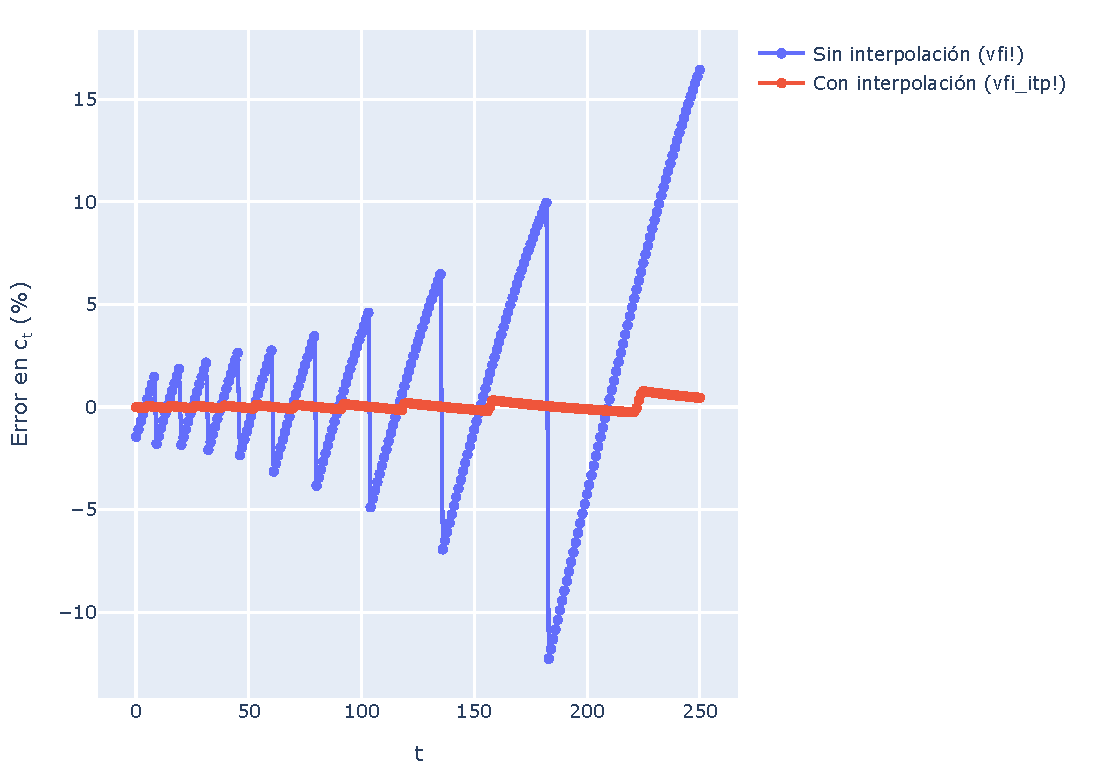
\includegraphics[width=\linewidth]{sim_err_c.pdf}\caption{Consumo}\end{subfigure}
\begin{subfigure}{.49\textwidth}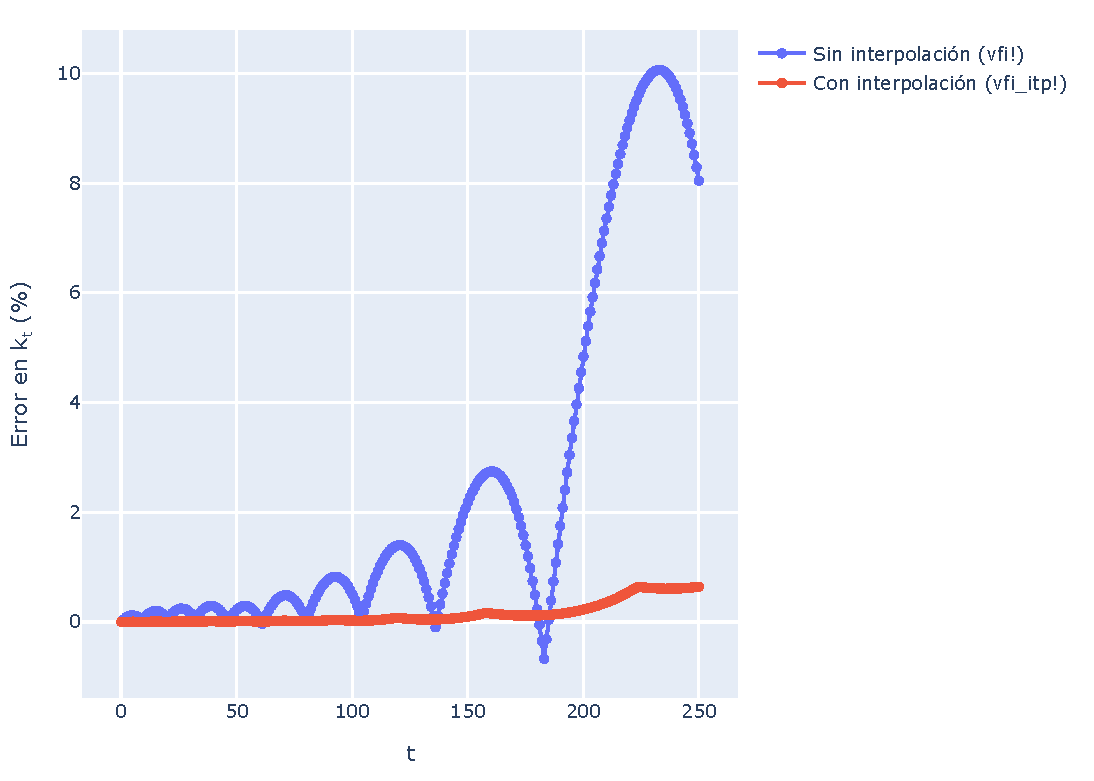
\includegraphics[width=\linewidth]{sim_err_k.pdf}\caption{Torta}\end{subfigure}
\caption{Error relativo de la trayectoria simulada respecto de la forma cerrada, $x_t/x_t^{\text{cerrada}}-1$, con $N_k=1000$.}
\label{fig:simerr}
\end{figure}

\begin{table}[H]
\centering
\begin{tabular}{lccccc}
\toprule
 & & & \multicolumn{2}{c}{Error en $c_t$ (\%)} & Error en $k_T$\\
\cmidrule(lr){4-5}
 & $c_0$ & $k_T$ & Máximo & Medio & (\%)\\
\midrule
Forma cerrada                   & 0.0305 & 0.0723 & -- & -- & --\\
Sin interpolación, $N_k=20$     & 0.0200 & 1.0000 & 808.76 & 227.54 & 1283.81\\
Con interpolación, $N_k=20$     & 0.0292 & 0.1839 & 100.38 & 28.45 & 154.44\\
Sin interpolación, $N_k=1000$   & 0.0300 & 0.0781 & 16.44 & 4.01 & 8.05\\
Con interpolación, $N_k=1000$   & 0.0305 & 0.0727 & 0.77 & 0.14 & 0.64\\
\bottomrule
\end{tabular}
\caption{Simulaciones con las reglas de los cuatro modelos resueltos en el inciso~\ref{sec:resolucion}, $T=250$ y $k_0=1$. Los errores en $c_t$ son el máximo y el promedio de $|c_t/c_t^{\text{cerrada}}-1|$ en los 251 períodos.}
\label{tab:sim}
\end{table}

En la Sección~\ref{sec:funciones} cada regla se evaluó en cada torta por separado, de modo que un error en un punto no afectaba a los demás. En la simulación, en cambio, la torta con la que el agente decide mañana es la que resulta de lo que comió hoy, y los errores pasan de un período al siguiente. La restricción presupuestaria lo muestra:
\[
k_{t+1}-k_{t+1}^{\text{cerrada}}=(1+r)\big(k_t-k_t^{\text{cerrada}}\big)-\big(c_t-c_t^{\text{cerrada}}\big).
\]
La diferencia de torta de mañana es la de hoy, con intereses, más lo que se comió de menos hoy. La torta acumula así los errores de consumo pasados con su signo: los períodos en que el agente come de menos la agrandan respecto de la teórica y los períodos en que come de más la achican. Sin interpolación y con $N_k=1000$, mientras la torta baja la misma cantidad de pasos por período el error de consumo mantiene su signo y la brecha de torta crece; cuando esa cantidad cambia, el signo se invierte y la brecha se cierra. Por eso el error de la torta forma arcos (Figura~\ref{fig:simerr}b), que vuelven casi a cero pero son cada vez más altos. Al final del horizonte la torta queda por encima de la teórica con los cuatro modelos (Cuadro~\ref{tab:sim}): un $8\%$ sin interpolación y un $0.6\%$ con interpolación con $N_k=1000$; y con $N_k=20$ un $154\%$ con interpolación con y sin interpolación la torta queda intacta.

El error en el consumo tiene dos componentes. Uno es el de la regla $c/k$ evaluada en la torta de cada período, que según los incisos~\ref{sec:consumorelativo} y~\ref{sec:ahorro} aumenta a medida que la torta se achica. El otro es heredado: con más torta que la teórica, el agente también consume más. Sin interpolación y con $N_k=1000$, el primero produce una oscilación (Figura~\ref{fig:simerr}a). Mientras la torta baja la misma cantidad de pasos por período, el consumo queda por debajo o por encima del óptimo, y cuando esa cantidad cambia, salta al otro lado. A medida que la torta se achica, un paso de grilla representa una parte mayor de ella, y la amplitud de la oscilación pasa de $\pm2\%$ en los primeros períodos a $16\%$ al final. Con interpolación el error se mantiene por debajo de $0.32\%$ durante los primeros 200 períodos y crece recién al final, hasta $0.77\%$, cuando la torta llega a la zona donde la regla es menos precisa. Como ambas componentes crecen con el tiempo, en los cuatro modelos el mayor error de consumo se alcanza en los últimos períodos.

\paragraph{Conclusión.} Con una regla precisa, la torta y el consumo caen el mismo porcentaje cada período, como en la forma cerrada. La simulación agrega a la Sección~\ref{sec:funciones} la dimensión temporal: al encadenar los períodos, lo que el agente come de más o de menos hoy cambia la torta con la que decide mañana. Por eso los errores se arrastran de un período al siguiente y, aunque oscilen, tanto el de la torta como el del consumo tienden a crecer con el tiempo. La regla del método discreto con 1000 puntos, que en el inciso~\ref{sec:ahorro} se apartaba de $\theta$ hasta un $7\%$ para $k\geq0.2$, termina generando un error de $16\%$ en el consumo después de 250 períodos.

\end{document}